% arara: pdflatex
% arara: showfile
\documentclass[border=0pt]{standalone}
\usepackage{tikzlings}
\usetikzlibrary{ducks}
\usetikzlibrary{shapes.geometric}
\definecolor{blueinter}{RGB}{0,102,170}%
\tikzset{
  linea/.style={white, line width=4pt,},
  pics/microph/.style={code={ 
        \draw[black, line width=.2em, rounded corners=1.7ex] 
            (-.85em,4.5ex) -- (-.85em,2ex) -- (.85em,2ex) -- (.85em,4.5ex);
        \fill[black] 
            (-.6em,5ex) to[rounded corners=1.2ex]  
            (-.6em,2.5ex) to[rounded corners=1.2ex] (.6em,2.5ex)
            -- (.6em,5ex) to[rounded corners=.2ex] ++(-.85em,0) to[rounded corners=.2ex] ++(0,.35ex) -- ++(.85em,0)  
            -- (.6em,5.5ex) to[rounded corners=.2ex] ++(-.85em,0) to[rounded corners=.2ex] ++(0,.35ex) -- ++(.85em,0)
            -- (.6em,6ex) to[rounded corners=.2ex] ++(-.85em,0) to[rounded corners=.2ex] ++(0,.35ex) -- ++(.85em,0)
            -- (.6em,6.5ex) to[rounded corners=.2ex] ++(-.85em,0) to[rounded corners=.2ex] ++(0,.35ex) -- ++(.85em,0)
            to[rounded corners=1.2ex]
            (.6em,8ex) to[rounded corners=1.2ex]
            (-.6em,8ex) to cycle; 
    }},
		Bear/.pic = {
			\begin{scope}
				\bear[magichat=blueinter,
					magicstars=black
					]
			\end{scope}},
		Cat/.pic = {
			\begin{scope}
				\cat[magichat=white,
					magicstars=black
					]
			\end{scope}},
		Coati/.pic = {
			\begin{scope}
				\coati
			\end{scope}},
		Hippo/.pic = {
			\begin{scope}
				\hippo[signpost=\scalebox{0.8}{%
						\parbox{2cm}{\color{black}
						\centering W\\ Juve!}},
					signcolour=white,
					signback=white]
			\end{scope}},
		Koala/.pic = {
			\begin{scope}
				\koala[
					harlequin=black,
					niuqelrah=blueinter]
			\end{scope}},
		Marmot/.pic = {
			\begin{scope}
				\marmot
			\end{scope}}, 
		Moles/.pic = {
			\begin{scope}
				\moles[signpost={},
					signpost=\scalebox{0.8}{%
						\parbox{2cm}{\color{black}
						\centering W\\ Inter!}},
					signcolour=blueinter,
					signback=blueinter]
			\end{scope}}, 
		Mouse/.pic = {
			\begin{scope}
				\mouse
			\end{scope}},
		Owl/.pic = {
			\begin{scope}
				\owl[
					strawhat=white,
					ribbon=black
					]
			\end{scope}},
		Panda/.pic = {
			\begin{scope}
				\panda[
					harlequin=black,
					niuqelrah=white]
			\end{scope}},
		Penguin/.pic = {
			\begin{scope}
				\penguin
			\end{scope}},
		Pig/.pic = {
			\begin{scope}
				\pig[
					strawhat=blueinter,
					ribbon=black
					]
			\end{scope}},
		Rhino/.pic = {
			\begin{scope}
				\rhino
			\end{scope}},
		Sloth/.pic = {
			\begin{scope}
				\sloth
			\end{scope}},
		Snowman/.pic = {
			\begin{scope}
				\snowman
			\end{scope}},
}
\begin{document}
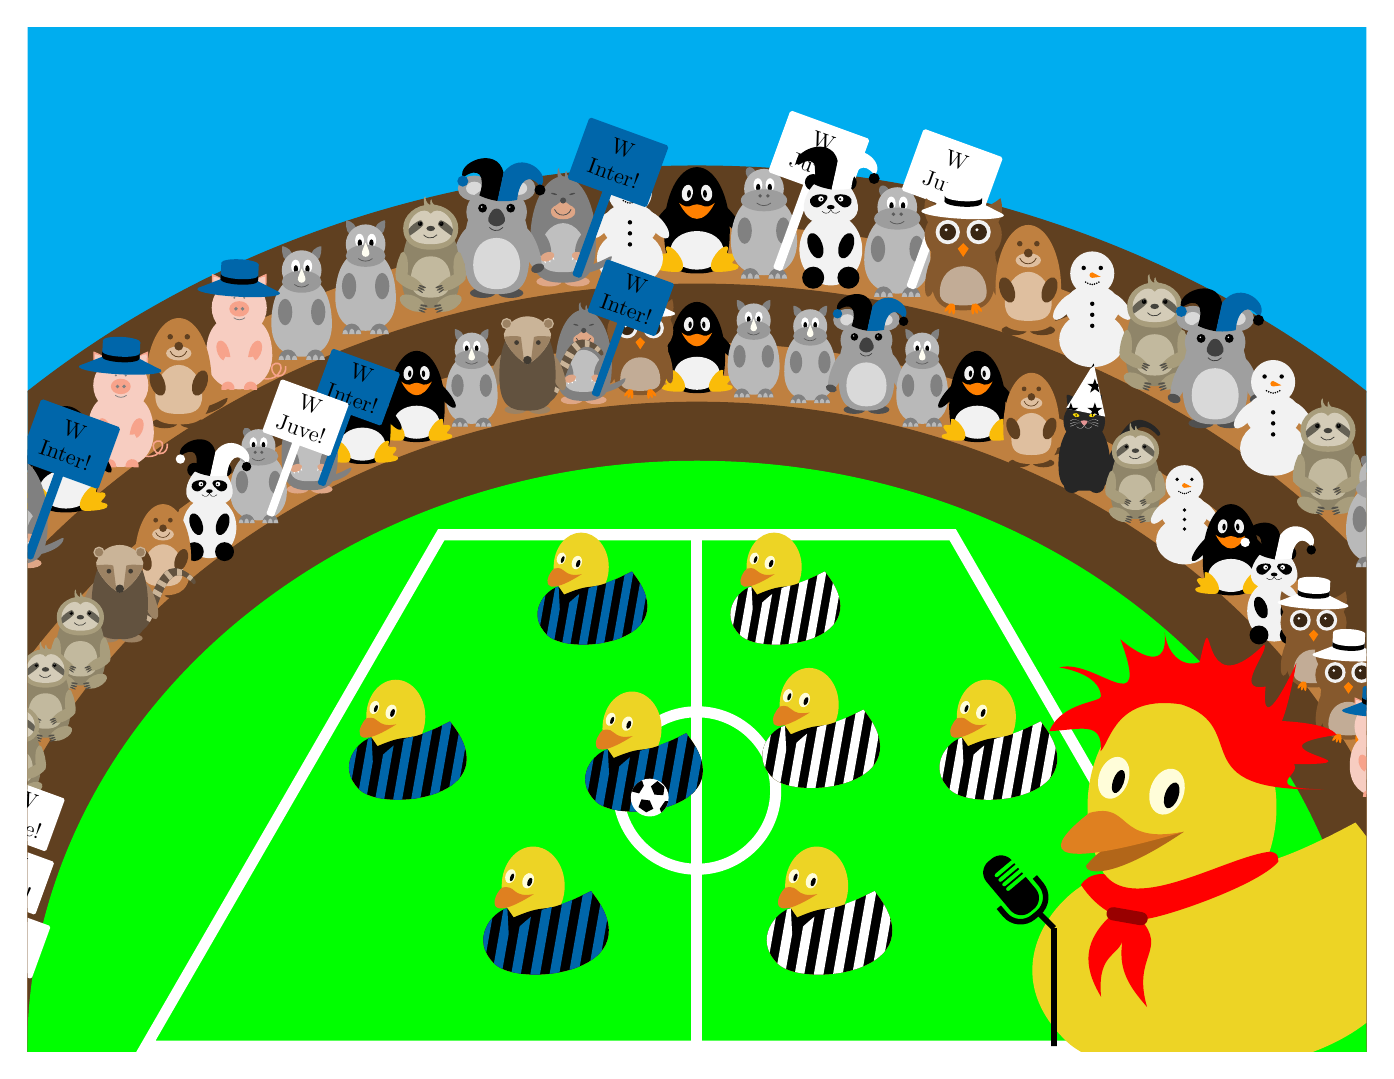
\begin{tikzpicture}
\begin{scope}
\pic[rotate=40, local bounding box=microfono] at (4.5,-5) {microph};
\clip (-8.5,-6.5) rectangle (8.5,6.5);
% background
\node[fill=cyan, draw=cyan, minimum width=17cm, minimum height=13cm](sky){};
\node[shape=ellipse, fill=brown!50!black, draw=brown!50!black, anchor=center,scale=1.5, minimum height=15cm, minimum width=17cm] at (sky.south) {};
\node[shape=ellipse, fill=brown, draw=brown, anchor=center,scale=1.4, minimum height=15cm, minimum width=17cm] at (sky.south) {};
\node[shape=ellipse, fill=brown!50!black, draw=brown!50!black, anchor=center,scale=1.3, minimum height=15cm, minimum width=17cm] (secondoanello) at (sky.south) {};
\node[shape=ellipse, fill=brown, draw=brown, anchor=center,scale=1.2, minimum height=15cm, minimum width=17cm] at (sky.south) {};
\node[shape=ellipse, fill=brown!50!black, draw=brown!50!black, anchor=center,scale=1.1, minimum height=15cm, minimum width=17cm] (primoanello) at (sky.south) {};
\node[shape=ellipse, fill=green, draw=green, anchor=center, minimum height=15cm, minimum width=17cm] at (sky.south) {};\node[shape=trapezium, fill=green, draw=white, line width=4pt, minimum width=14cm, anchor=south] (field) at (sky.south) {};
\draw[linea] (field.north) -- (field.south);
\draw[linea] (field.center) circle (1cm);

% soccer players
\duck[tshirt=black,scale=.7,shift={(-3,-2)},
stripes={\stripes[color=blueinter,]}
]
\duck[tshirt=black,scale=.75,shift={(-6,-4.5)},
stripes={\stripes[color=blueinter,]}
]
\duck[tshirt=black,scale=.75,shift={(-2,-4.7)},
stripes={\stripes[color=blueinter,]},
football
]
\duck[tshirt=black,scale=.8,shift={(-3.5,-7)},
stripes={\stripes[color=blueinter,]}
]

\duck[tshirt=black,scale=.7,shift={(.5,-2)},
stripes={\stripes[color=white,]}
]
\duck[tshirt=black,scale=.75,shift={(4,-4.5)},
stripes={\stripes[color=white,]}
]
\duck[tshirt=black,scale=.75,shift={(1,-4.3)},
stripes={\stripes[color=white,]}
]
\duck[tshirt=black,scale=.8,shift={(1,-7)},
stripes={\stripes[color=white,]}
]
% soccer fans
\pgfmathdeclarerandomlist{randomling}{{Cat}{Coati}{Hippo}{Koala}{Marmot}{Moles}% 
	{Mouse}{Owl}{Panda}{Penguin}{Pig}{Rhino}{Sloth}{Snowman}}
\foreach \grado in {90,85,...,0} {
	\pgfmathrandomitem{\randomling}{randomling}
	\pic[scale=.7,
		] at (secondoanello.\grado) {\randomling};	
	}
\foreach \grado in {90,85,...,0} {
	\pgfmathrandomitem{\randomling}{randomling}
	\pic[scale=.6,
		] at (primoanello.\grado) {\randomling};
	}
\foreach \grado in {95,100,...,180} {
	\pgfmathrandomitem{\randomling}{randomling}
	\pic[scale=.7,
		] at (secondoanello.\grado) {\randomling};	
	}
\foreach \grado in {95,100,...,180} {
	\pgfmathrandomitem{\randomling}{randomling}
	\pic[scale=.6,
		] at (primoanello.\grado) {\randomling};
	}
% Gianna 
\pic[scale=2.4,
	duck/laughing,
	duck/neckerchief=red,
	duck/crazyhair=red,
	duck/woggle=red!60!black
	] at (4,-7) {duck};
	\pic[rotate=40] at (4.5,-5) {microph};
	\draw[black, line width=2pt] (microfono.-45) -- ++(-.2,+.2) ++(.2,-.2) -- ++(0,-1.5);
\end{scope}
\end{tikzpicture}
\end{document}
